\documentclass[xcolor=dvipsnames]{beamer}
\usepackage{graphicx}
\usepackage{amsmath}
\usepackage{amssymb}   
\usepackage{graphicx}
\usetheme{default}
\usecolortheme[named=Green]{structure}
\usepackage{algpseudocode}
\newcommand{\bb}[1]{\textbf{#1}}



\DeclareMathOperator*{\argmin}{arg\,min}


\title{Bertozzi Meeting 4/14}
\author{Charlie Marshak}
\date{April 2014}

\begin{document}
\begin{frame}
\begin{large}
\begin{center}
Dynamic Preferential Tree Growth And Criminal Pursuit
\end{center}
\end{large}
\end{frame}

\begin{frame}{Part I: Dynamic Preferential Tree Growth}
Let $\bb T^t$ be the tree at time $t$. We set $\bb T^0 = $ root, dubbed Pablo.
\\

\begin{itemize}
\item The process is recursive.  To obtain $\bb T^t$ from $\bb T^{t-1}$, $k$ new nodes are added to $\bb T^{t-1}$.  Each new node will be attached to an existing node $j$ in $\bb T^{t-1}$ with probability proportional to weight $w(j, t-1)$.  We set:
\begin{center}
\framebox{$w(j, t-1) =$ {the weight of node j} $\displaystyle{= \frac{1}{d(j, \mathcal{L}_{t-1})+1}}$}
\end{center}
where $\mathcal{L}_{t-1} = $ set of leaves at time $t-1$ and $d$ denotes the minimum distance via a directed path in $\bb T^{t-1}$.  In this case, the path's from node $j$ to the set $\mathcal{L}_{t-1}$.
\end{itemize}

\end{frame}


\begin{frame}{Degree Distribution}

\begin{figure}
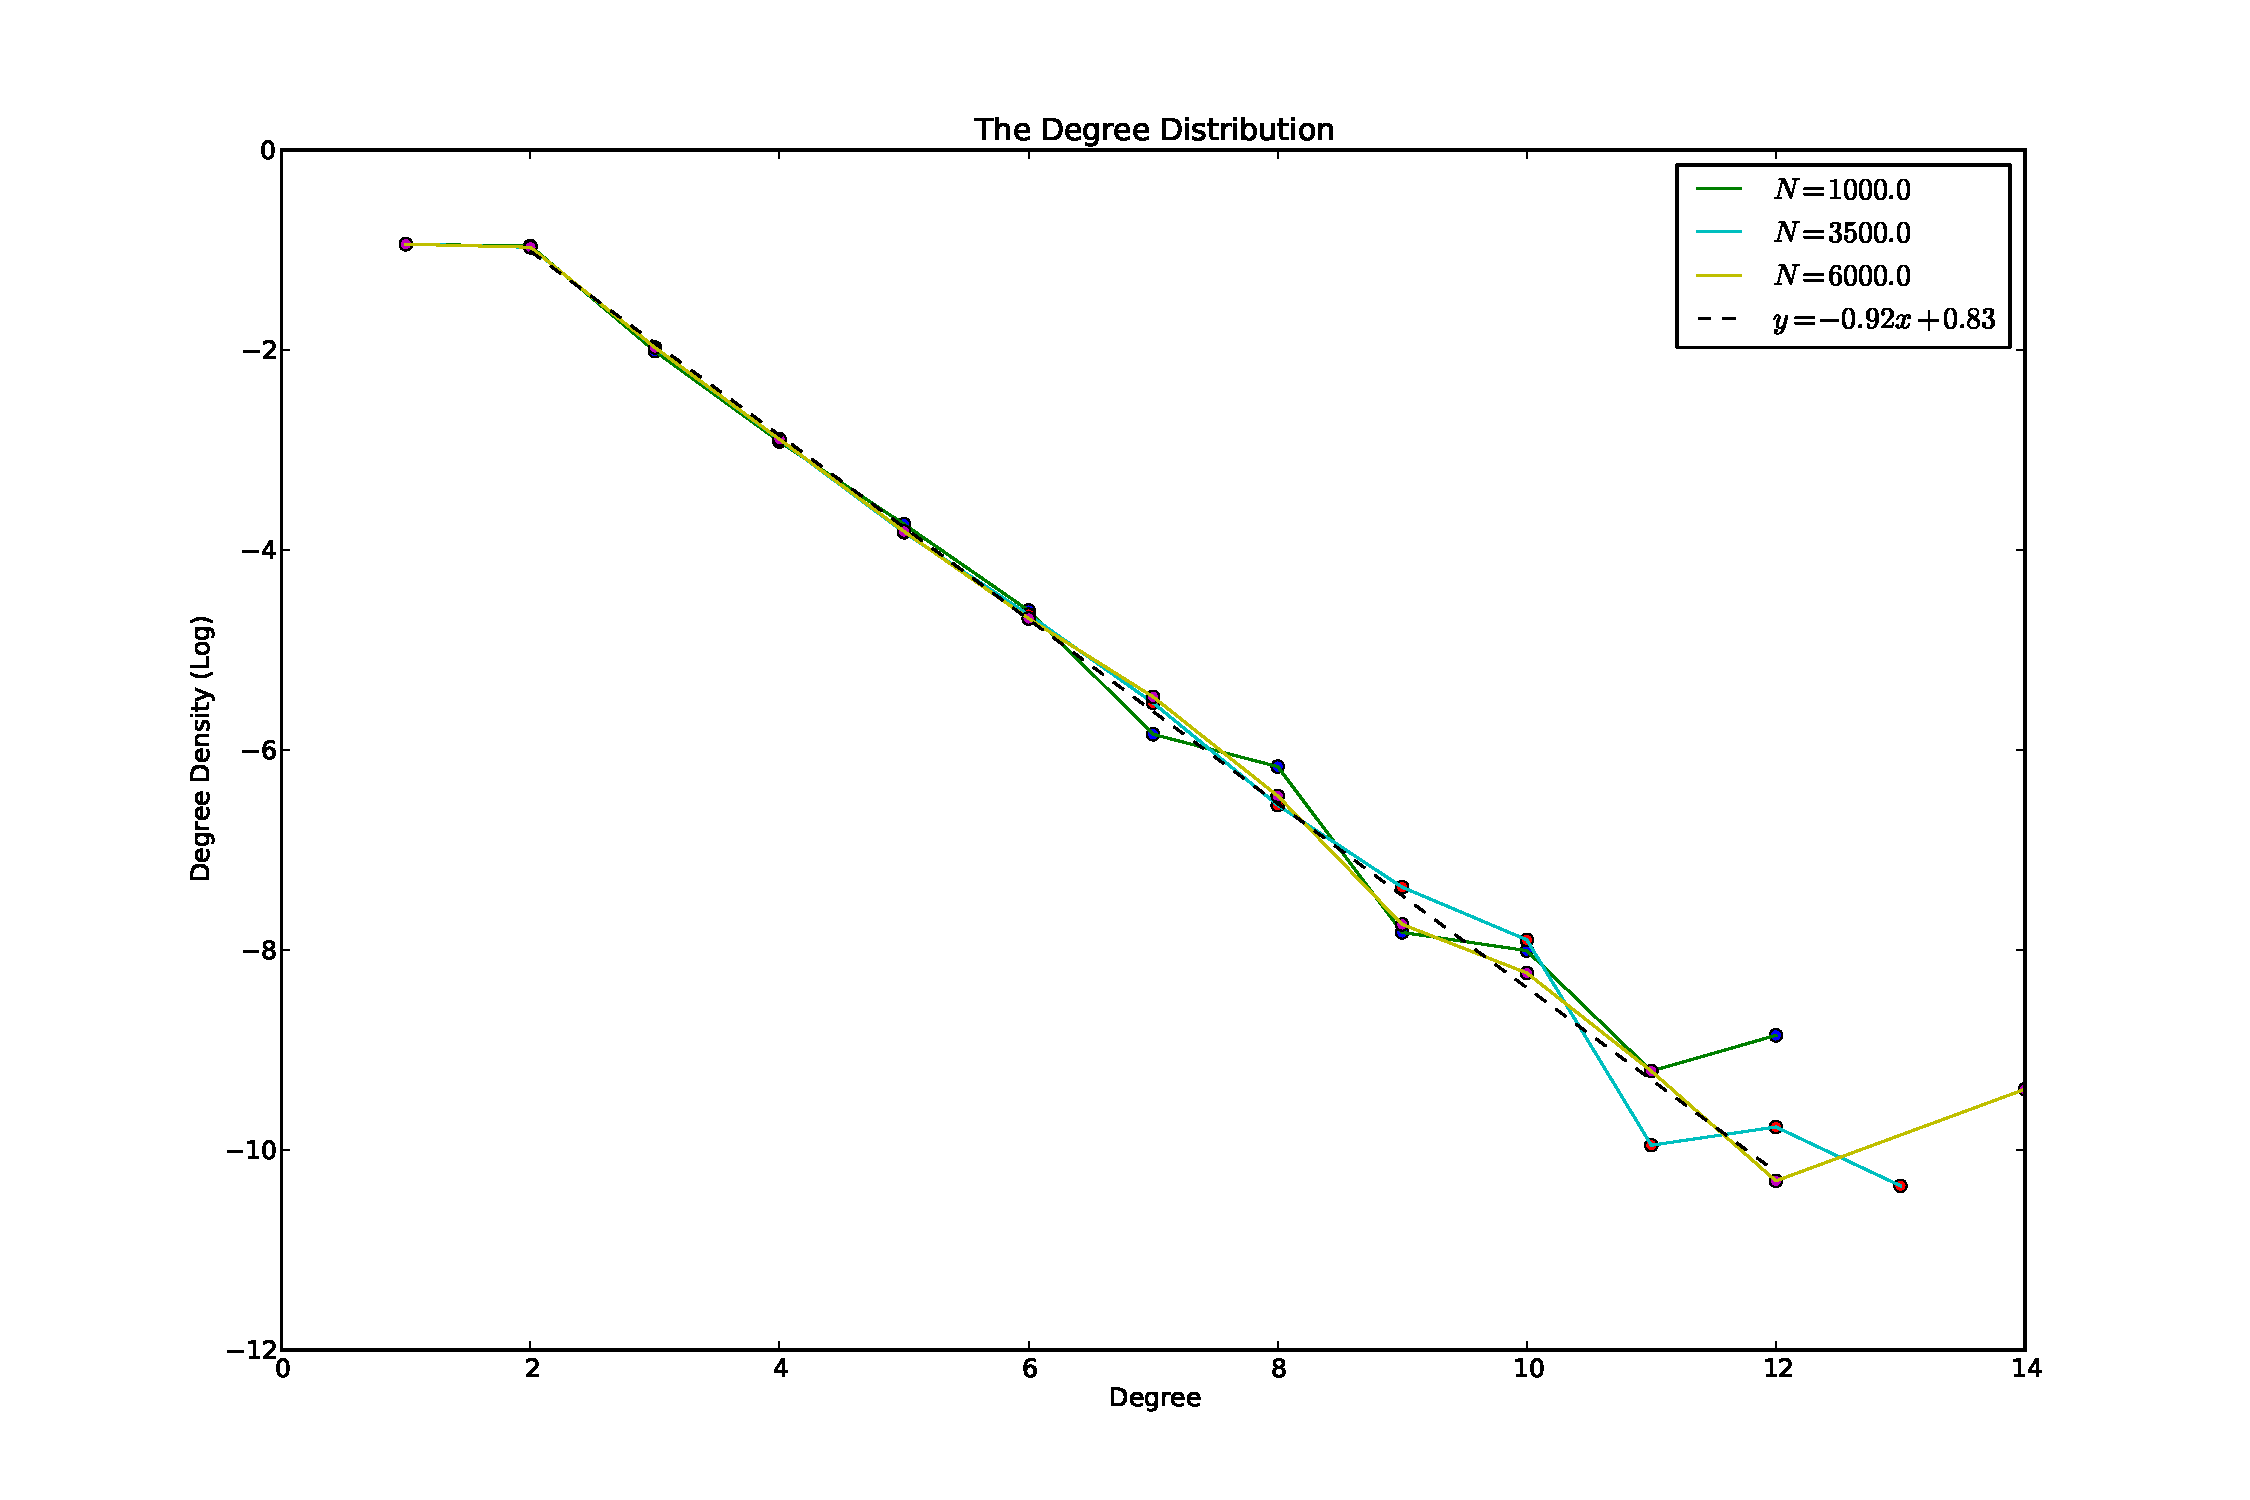
\includegraphics[width = 3.5in]{DDPEAKLog.pdf}
\caption{The Degree Density is given by $\bb P($node has degree $d)$}
\end{figure}
\end{frame}


\begin{frame}{Node Density}
\begin{figure}
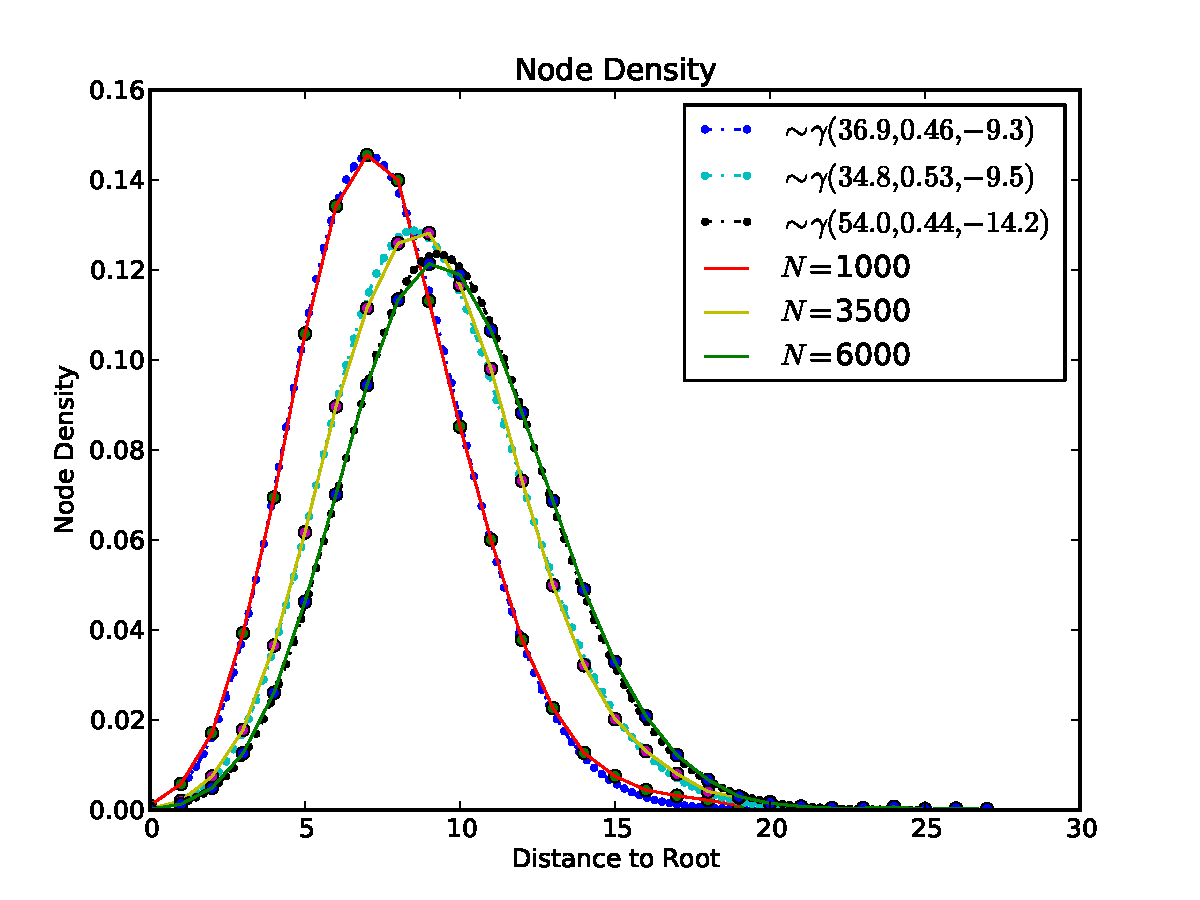
\includegraphics[width = 2.75in]{NodeDensity.pdf}
\caption{Node density is the probability that a randomly selected node is at a given height.  We performed a single experiment for the above data. $\gamma(\alpha, \beta, s)$ is the fitted gamma distribution with translation parameter $s$.}
\end{figure}
\end{frame}

\begin{frame}{The Gamma Distribution}

\begin{itemize}\item Let $S_{\alpha, \beta}$ be $\gamma$ distributed random variable.  The density of the gamma distribution is given by:
$$
\rho_{\alpha, \beta}(x) = \frac{\beta^\alpha}{\Gamma(\alpha)}x^{\alpha-1}e^{ -\beta x}
$$
\item If $\alpha = n \in \mathbb{N}$ and $\beta = \lambda \in \mathbb R^+$, then the interpretation of $S_{n, \lambda}$ is as follows: if $X_1, \hdots, X_n$ are iid exponential random variables with parameter $\lambda$, then:
$$
S_{n, \lambda}= X_{1}+ \hdots + X_{n}
$$
\item In the current situation, we add a parameter $s$, namely the gamma distribution is of the form $S_{\alpha, \beta, s}:= S_{\alpha, \beta}+ s$, where $s$ is a constant.  This simply translates the density function.

\end{itemize}

\end{frame}



\begin{frame}{Conjectures on Growth}
\begin{enumerate}
\item The Node Density is a gamma distributed random variable $S_{\alpha, \beta, s}$ where $\alpha, \beta, s$ depend on the rate of arrival $k$, the maximum number of nodes before the process stops $N$, and the weight function $w$.
\item The degree distribution of the tree obeys an exponential law where $\bb P($node has degree $d) = e^{-m d}$, with $m>0$.
\end{enumerate}
\end{frame}

\begin{frame}{An Example of Growth}
\begin{figure}
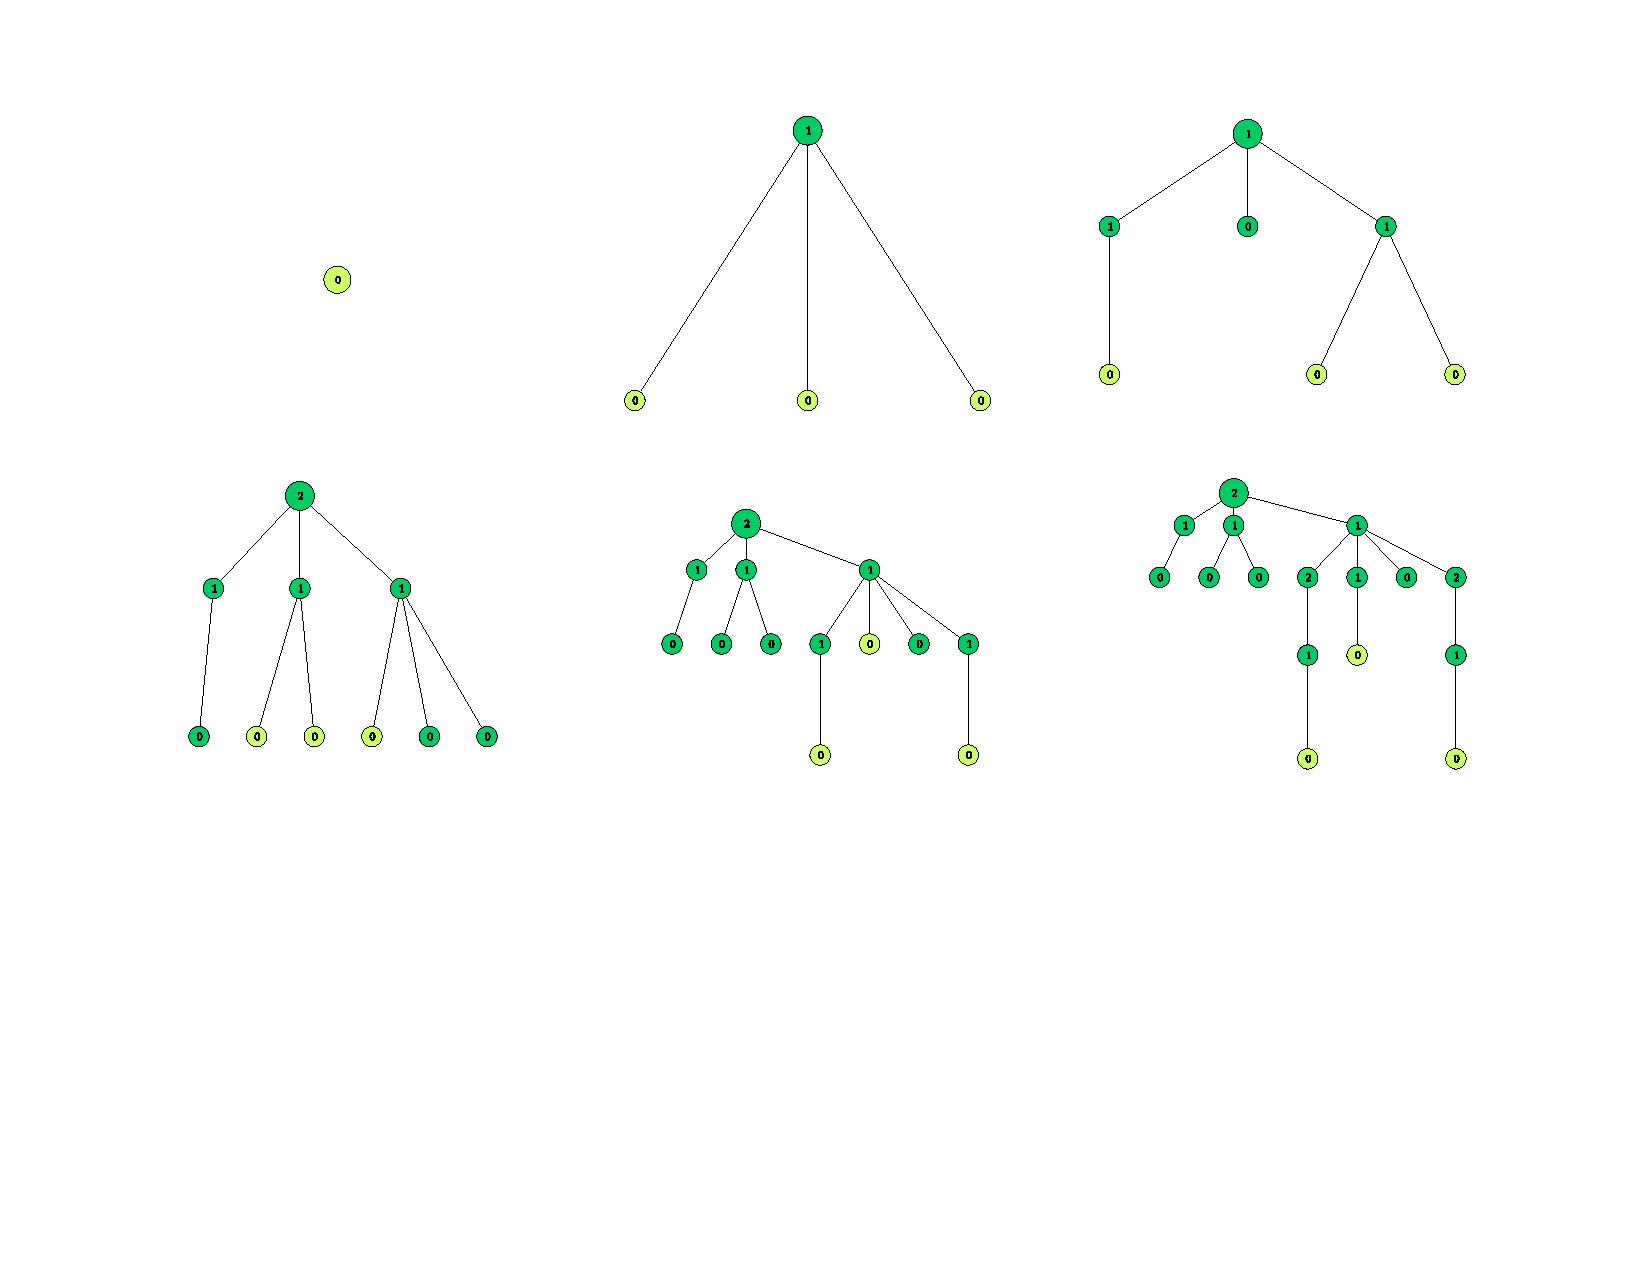
\includegraphics[width = 4in]{GrowthPic.pdf}
\caption{We see the growth for time steps $0 \leq t \leq 5$ and $k= 3$.  We have labeled $d(j, \mathcal L)$ on each node.  The yellow nodes are the new nodes added at the time step.}
\end{figure}
\end{frame}

\begin{frame}{Part II: The Criminal Pursuit}

We begin with uniform complete $k$-ary tree as the seed. We set $\bb T^0=$ seed.  Let $\bb T^{t}$ be the tree at time $t$.

\begin{enumerate}
\item $\bb T^{t+1/2}$:  We place $k-k^*$ officers on the leaves where $k$ is the arrival rate specified in the model and $k^* \geq 0$ (note when $k^* < 0$, the police always have a winning strategy).  The officer can:
\begin{itemize}
\item Move in a self-avoiding walk (investigate)
\item Remove a node and all of its children (arrest)
\end{itemize}
If the officer reaches the root, the game is over.  Should the officer reach another leaf in his walk, he must give up his investigation and wait until a future round.
\item  $\bb T^{t+1}$: the dynamic growth described earlier is performed with arrival rate $k$.
\end{enumerate}

\end{frame}

\begin{frame}{Conjectures about Pursuit}

\begin{enumerate}
%[label=(\roman*)]
\item Let $S$ be a police strategy regarding whether to investigate or arrest.  Let:
$$
\textrm{Beat}(S) := \max{(k^* | \textrm{police arrests Pablo in finite time}})
$$
Let $S_1$ be the strategy of arresting only and $S_2$ be the strategy of investigating only.  Then, there exists a $S' = C(S_1, S_2)$, a  combination of $S_1$ and $S_2$ such that
$$
\textrm{Beat}(C(S_1, S_2)) > \max(\textrm{Beat}(S_1), \textrm{Beat}(S_2))
$$
Moreover $C(S_1, S_2)$ depends only on \textit{local} information (degree) and the length of the walk.
\item There exists a bad strategy $S$ such that:
$$
\textrm{Beat}(S) < \min (\textrm{Beat}(S_1), \textrm{Beat}(S_2))
$$
\end{enumerate}
\end{frame}

%
%\begin{frame}{Appendix}
%The trend is a little bit more subtle.
%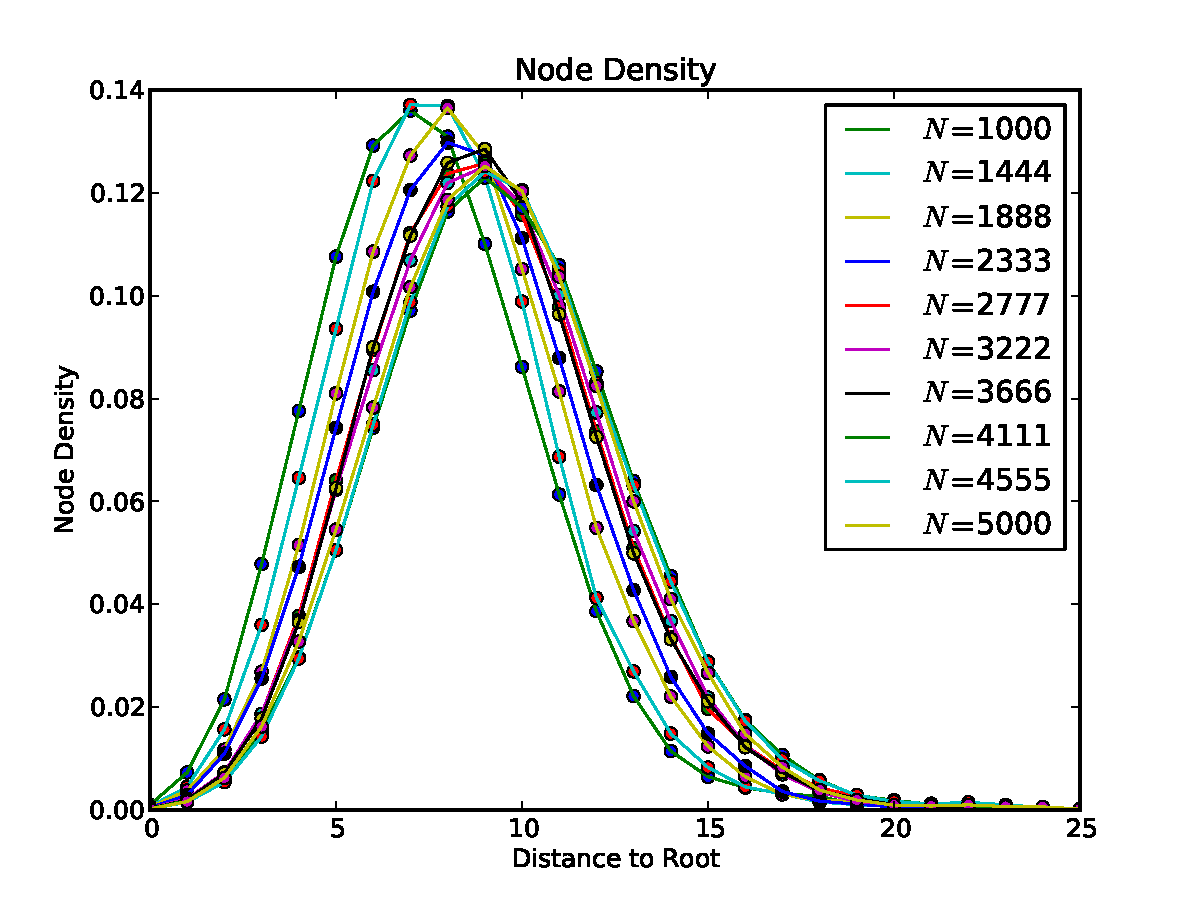
\includegraphics[width = 3 in ]{PEAKTEST!.pdf}
%\end{frame}

\end{document}
